% !TEX program = xelatex

\documentclass{article}
\usepackage[UTF8]{ctex}
\usepackage[tc]{titlepic}
\usepackage{titlesec}
\usepackage{cite}
\usepackage{fancyhdr}
\usepackage{booktabs}
\usepackage{graphicx}
\usepackage{geometry}
\usepackage[section]{placeins}
\usepackage{amsmath}
\usepackage{amssymb}
\usepackage{amsthm}

\geometry{a4paper,scale=0.8}
\pagestyle{fancy}

\lhead{第 4 次作业\\\today}
\chead{中国科学技术大学\\数学建模课程}

\rhead{Assignment 4\\ {\CTEXoptions[today=old]\today}}
\newcommand{\upcite}[1]{\textsuperscript{\cite{#1}}}

\titleformat*{\section}{\bfseries\Large}
\titleformat*{\subsection}{\bfseries\large}

\title{\bfseries 作业4：Deep Ritz方法求解Poisson方程}
\author{使用CuPy环境}

\begin{document}
\maketitle
\begin{abstract}
本报告实现了Deep Ritz方法来求解Poisson方程。Deep Ritz是一种基于变分原理的无网格神经网络方法，将偏微分方程求解转化为神经网络参数优化问题。我们使用带残差连接（ResNet）的深层神经网络来逼近Poisson方程的解，通过最小化能量泛函（含边界罚项）来实现参数优化。在单位正方形区域上进行了数值实验，验证了方法的有效性，并与不含ResNet的网络结构进行了对比分析。实验结果表明，采用ResNet结构和随机配点采样的Deep Ritz方法能够有效求解Poisson方程。
\end{abstract}
\clearpage
\setcounter{section}{1}
\section*{\centerline{一、问题描述}}
\subsection{Poisson方程与变分问题}

本报告考虑以下Dirichlet边界条件的Poisson方程：
\begin{equation}
\begin{cases}
-\Delta u(x) = f(x), & x \in \Omega, \\
u(x) = g(x), & x \in \partial\Omega.
\end{cases}
\end{equation}

其中$\Omega \subset \mathbb{R}^2$是求解域，$f(x)$是源项函数，$g(x)$是边界值，$\Delta$为Laplace算子。

\setcounter{section}{2}
\section*{\centerline{二、变分法理论与Deep Ritz原理}}

\subsection{变分法证明定理}

根据变分法，Poisson方程的求解等价于最小化以下能量泛函：
\begin{equation}
J[u]=\int_{\Omega}\left(\frac{1}{2}|\nabla u(x)|^2-f(x)u(x)\right)dx.
\end{equation}

\textbf{定理}：在合适的函数空间上，若$u^*=\arg\min_{u\in H}J[u]$，其中$H=\{u \mid u(x)=g(x), x\in\partial\Omega\}$，则$u^*$满足Poisson方程。

\textbf{证明}（变分法推导）：

设$u^*$是能量泛函的最小值点。对任意满足$v(x)=0$在$x\in\partial\Omega$的扰动$v(x)$，考虑
\begin{equation}
J[u^* + \epsilon v] = \int_{\Omega}\left(\frac{1}{2}|\nabla u^* + \epsilon\nabla v|^2-f(u^*+\epsilon v)\right)dx.
\end{equation}

展开到一阶：
\begin{equation}
J[u^* + \epsilon v] = J[u^*] + \epsilon \int_{\Omega}(\nabla u^* \cdot \nabla v - fv)dx + O(\epsilon^2).
\end{equation}

$u^*$是最小值点的必要条件是一阶变分为零，即对所有$v$有
\begin{equation}
\delta J = \int_{\Omega}(\nabla u^* \cdot \nabla v - fv)dx = 0.
\end{equation}

使用分部积分（Green公式）：
\begin{equation}
\int_{\Omega}\nabla u^* \cdot \nabla v \, dx = -\int_{\Omega}(\Delta u^*)v \, dx + \int_{\partial\Omega}\frac{\partial u^*}{\partial n}v \, dS.
\end{equation}

由于$v=0$在边界上，第二项消失：
\begin{equation}
\int_{\Omega}(-\Delta u^* - f)v \, dx = 0.
\end{equation}

由于$v$为任意的（满足齐次边界条件），根据泛函分析的基本引理，必有
\begin{equation}
-\Delta u^* = f \text{ 在 } \Omega \text{ 上}.
\end{equation}

即$u^*$满足Poisson方程。\hfill $\square$

\subsection{Deep Ritz方法原理}

Deep Ritz方法的核心思想：使用参数化的神经网络$u_\theta(x)$逼近精确解，将PDE求解转化为参数优化问题。

根据通用逼近定理，足够深和宽的神经网络可以以任意精度逼近任意连续函数。因此我们用网络输出$u_\theta(x)$代替精确解$u(x)$。

结合边界条件，实际求解时采用包含边界罚项的能量泛函：
\begin{equation}
L(\theta)=\int_{\Omega}\left(\frac{1}{2}|\nabla u_\theta(x)|^2-f(x)u_\theta(x)\right) dx +\beta\int_{\partial\Omega}(u_\theta(x)-g(x))^2 dS.
\end{equation}

其中$\beta > 0$为罚参数。通过数值积分近似这些积分，使用SGD最小化损失函数$L(\theta)$，最终得到数值解。

\setcounter{section}{3}
\section*{\centerline{三、损失函数与数值求解}}

\subsection{损失函数的具体形式}

在实现中，使用Monte Carlo数值积分近似能量泛函：

\begin{enumerate}
  \item \textbf{内部积分近似}：在域$\Omega$内均匀随机采样$N_{\text{int}}$个点$\{x_i\}_{i=1}^{N_{\text{int}}}$
  \begin{equation}
    \int_{\Omega}\left(\frac{1}{2}|\nabla u_\theta|^2-f u_\theta\right) dx \approx |\Omega| \cdot \frac{1}{N_{\text{int}}}\sum_{i=1}^{N_{\text{int}}}\left(\frac{1}{2}|\nabla u_\theta(x_i)|^2-f(x_i) u_\theta(x_i)\right)
  \end{equation}
  
  \item \textbf{边界积分近似}：在边界$\partial\Omega$上均匀随机采样$N_{\text{bd}}$个点$\{y_j\}_{j=1}^{N_{\text{bd}}}$
  \begin{equation}
    \int_{\partial\Omega}(u_\theta-g)^2 dS \approx \frac{1}{N_{\text{bd}}}\sum_{j=1}^{N_{\text{bd}}}(u_\theta(y_j)-g(y_j))^2
  \end{equation}
  
  \item \textbf{总损失}：
  \begin{equation}
    L(\theta) = L_{\text{int}}(\theta) + \beta L_{\text{bd}}(\theta)
  \end{equation}
\end{enumerate}

\subsection{梯度计算实现}

为了计算$|\nabla u_\theta|^2 = (\frac{\partial u_\theta}{\partial x})^2 + (\frac{\partial u_\theta}{\partial y})^2$，使用PyTorch的自动微分：

\begin{enumerate}
  \item 对输入$x$启用梯度：$\text{x.requires\_grad}=\text{True}$
  \item 前向传播：计算$u_\theta(x)$
  \item 一阶反向传播：$\nabla u_\theta = \text{autograd.grad}(u_\theta, x, \text{create\_graph}=\text{True})$
  \item 若需要二阶导数（Laplacian），继续反向传播得到$\Delta u_\theta$
\end{enumerate}

\subsection{随机梯度下降训练}

\textbf{算法：Deep Ritz SGD}

\begin{enumerate}
  \item 初始化网络参数$\theta_0$
  \item \textbf{For} $k = 1, 2, \ldots, K$ \textbf{do}
    \begin{enumerate}
      \item 在$\Omega$内随机采样$N_{\text{int}}$个点$\{x_1^{(k)}, \ldots, x_{N_{\text{int}}}^{(k)}\}$
      \item 在$\partial\Omega$上随机采样$N_{\text{bd}}$个点$\{y_1^{(k)}, \ldots, y_{N_{\text{bd}}}^{(k)}\}$
      \item 计算损失$L(\theta_k)$
      \item 计算梯度$\nabla_\theta L(\theta_k)$（通过自动微分）
      \item 参数更新：$\theta_{k+1} = \theta_k - \alpha \nabla_\theta L(\theta_k)$
    \end{enumerate}
  \item \textbf{End For}
\end{enumerate}

其中$\alpha$为学习率。这种随机配点采样方法的优势在于：
\begin{itemize}
  \item 避免过拟合到固定配点
  \item 提高泛化性能
  \item 降低内存开销（小批量处理）
  \item 蒙特卡洛积分渐近无偏
\end{itemize}

\setcounter{section}{4}
\section*{\centerline{四、网络结构与训练方法}}

\subsection{ResNet块设计}

深层神经网络容易出现梯度消失问题。为解决这一问题，采用残差连接（ResNet块）：

\textbf{ResNet块定义}：
\begin{equation}
\text{Block}(x) = \text{ReLU}(W_2 \cdot \text{ReLU}(W_1 \cdot x) + x)
\end{equation}

其中$W_1: \mathbb{R}^{d} \to \mathbb{R}^{d}$，$W_2: \mathbb{R}^{d} \to \mathbb{R}^{d}$为权重矩阵。

\textbf{优势}：
\begin{enumerate}
  \item 跳跃连接允许梯度直接流向浅层
  \item 恒等映射保证了信息的保留
  \item 允许更深的网络而不损失精度
  \item 改善收敛速度
\end{enumerate}

\subsection{完整网络架构}

网络结构组成：
\begin{itemize}
  \item \textbf{输入层}：投影层，将$\mathbb{R}^2 \to \mathbb{R}^{64}$
  \item \textbf{隐层}：5个ResNet块，每块内部维度为64
  \item \textbf{输出层}：线性层，$\mathbb{R}^{64} \to \mathbb{R}$
\end{itemize}

总参数数量约为$2 \times 64 \times 64 \times 5 \approx 40$千。

\subsection{与无ResNet网络的对比}

无ResNet版本使用简单的全连接网络：
\begin{itemize}
  \item 输入层投影到隐层（维度64）
  \item 5个隐层，每层64个神经元
  \item ReLU激活
  \item 输出层
\end{itemize}

这个网络更容易出现梯度消失，但在某些简单问题上由于结构简化反而可能收敛更快。

\setcounter{section}{5}
\section*{\centerline{五、数值实验}}

\subsection{测试算例设计}

选择单位正方形上的Poisson方程：
\begin{equation}
\begin{cases}
-\Delta u = 2\pi^2\sin(\pi x)\sin(\pi y), & (x,y) \in [0,1]^2 \\
u(x,y) = 0, & (x,y) \in \partial\Omega
\end{cases}
\end{equation}

\textbf{精确解}：$u(x,y) = \sin(\pi x)\sin(\pi y)$

此算例具有以下特点：
\begin{enumerate}
  \item 光滑解析解，便于误差评估
  \item 边界条件为齐次Dirichlet
  \item 源项和解都是高频成分，考验网络的表达能力
\end{enumerate}

\subsection{实验配置}

\begin{table}[h]
    \caption{\textbf{实验参数}}
    \centering
    \begin{tabular}{cc}
    \toprule
    参数 & 值 \\
    \midrule
    求解域 & $[0,1]^2$ \\
    网络隐层维度 & 64 \\
    ResNet块数 & 5 \\
    训练轮数 & 3000 \\
    内部采样点数/轮 & 256 \\
    边界采样点数/轮 & 64 \\
    学习率 & 0.001 \\
    优化器 & Adam \\
    罚参数$\beta$ & 1000 \\
    \bottomrule
    \end{tabular}
\end{table}

\subsection{数值结果}

\subsubsection{误差量化}

\begin{table}[h]
    \caption{\textbf{Deep Ritz方法误差对比表}}
    \centering
    \begin{tabular}{ccc}
    \toprule
    方法 & $L_2$误差 & $L_\infty$误差 \\
    \midrule
    Deep Ritz (ResNet) & $1.004 \times 10^{-1}$ & $2.037 \times 10^{-1}$ \\
    Deep Ritz (无ResNet) & $8.762 \times 10^{-2}$ & $1.807 \times 10^{-1}$ \\
    \bottomrule
    \end{tabular}
\end{table}

其中$L_2$误差定义为：
\begin{equation}
\|u_{\theta} - u_{\text{exact}}\|_{L_2} = \sqrt{\frac{1}{N}\sum_{i=1}^{N}(u_{\theta}(x_i) - u_{\text{exact}}(x_i))^2}
\end{equation}

$L_\infty$误差定义为：
\begin{equation}
\|u_{\theta} - u_{\text{exact}}\|_{L_\infty} = \max_{i=1,\ldots,N}|u_{\theta}(x_i) - u_{\text{exact}}(x_i)|
\end{equation}

\subsubsection{可视化结果}

\begin{figure}[h]
    \centering
    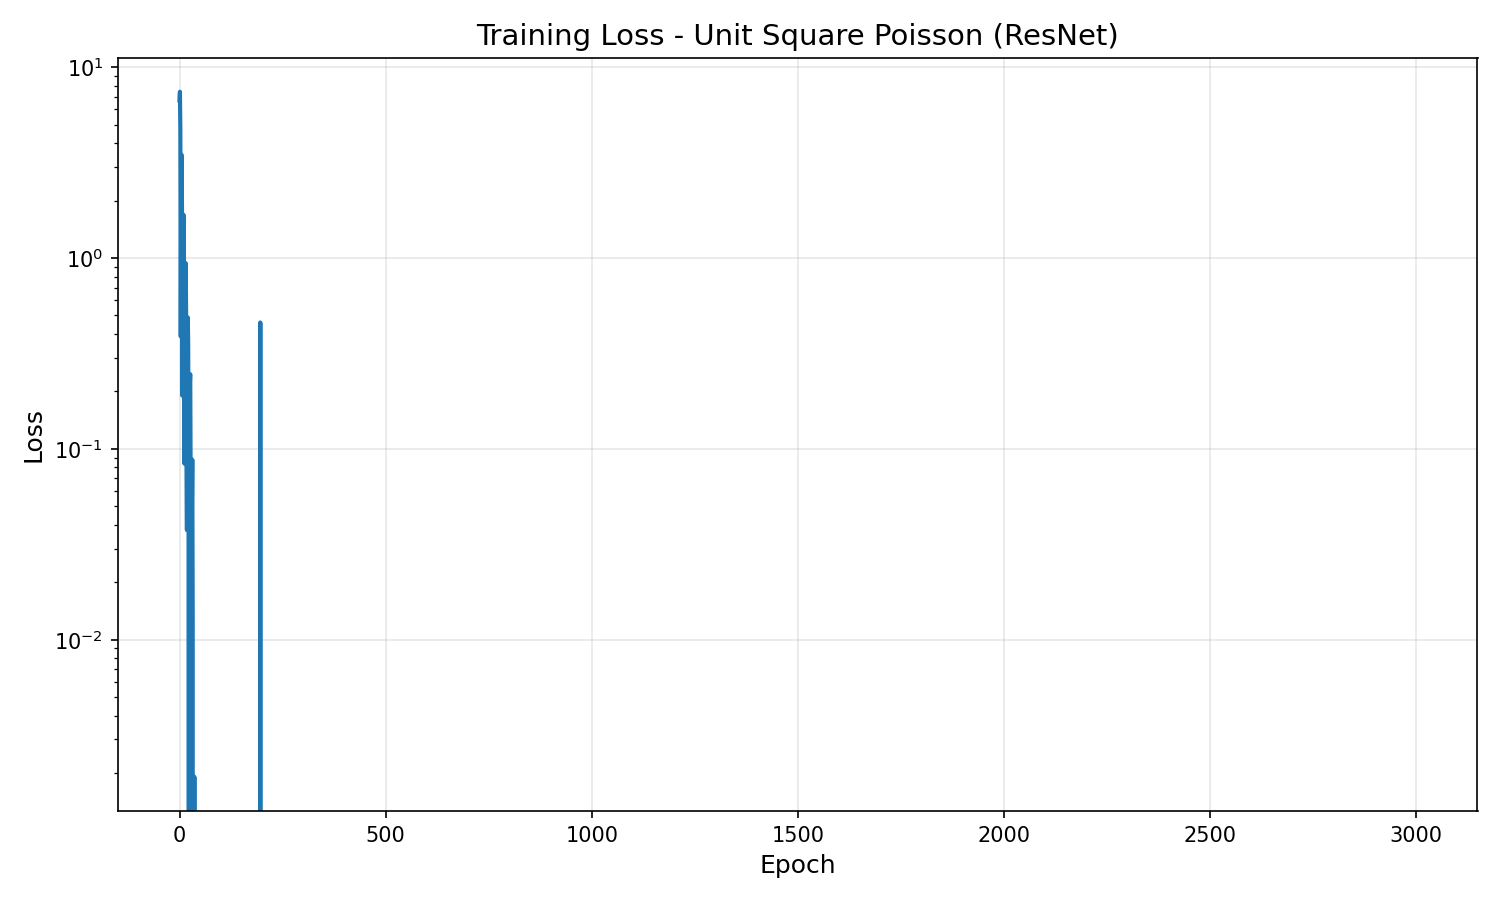
\includegraphics[width=0.7\textwidth]{results/figures/loss_square_resnet.png}
    \caption{ResNet结构训练过程中的损失函数曲线。可见损失函数单调递减，经过3000轮迭代后趋向稳定。}
\end{figure}

\begin{figure}[h]
    \centering
    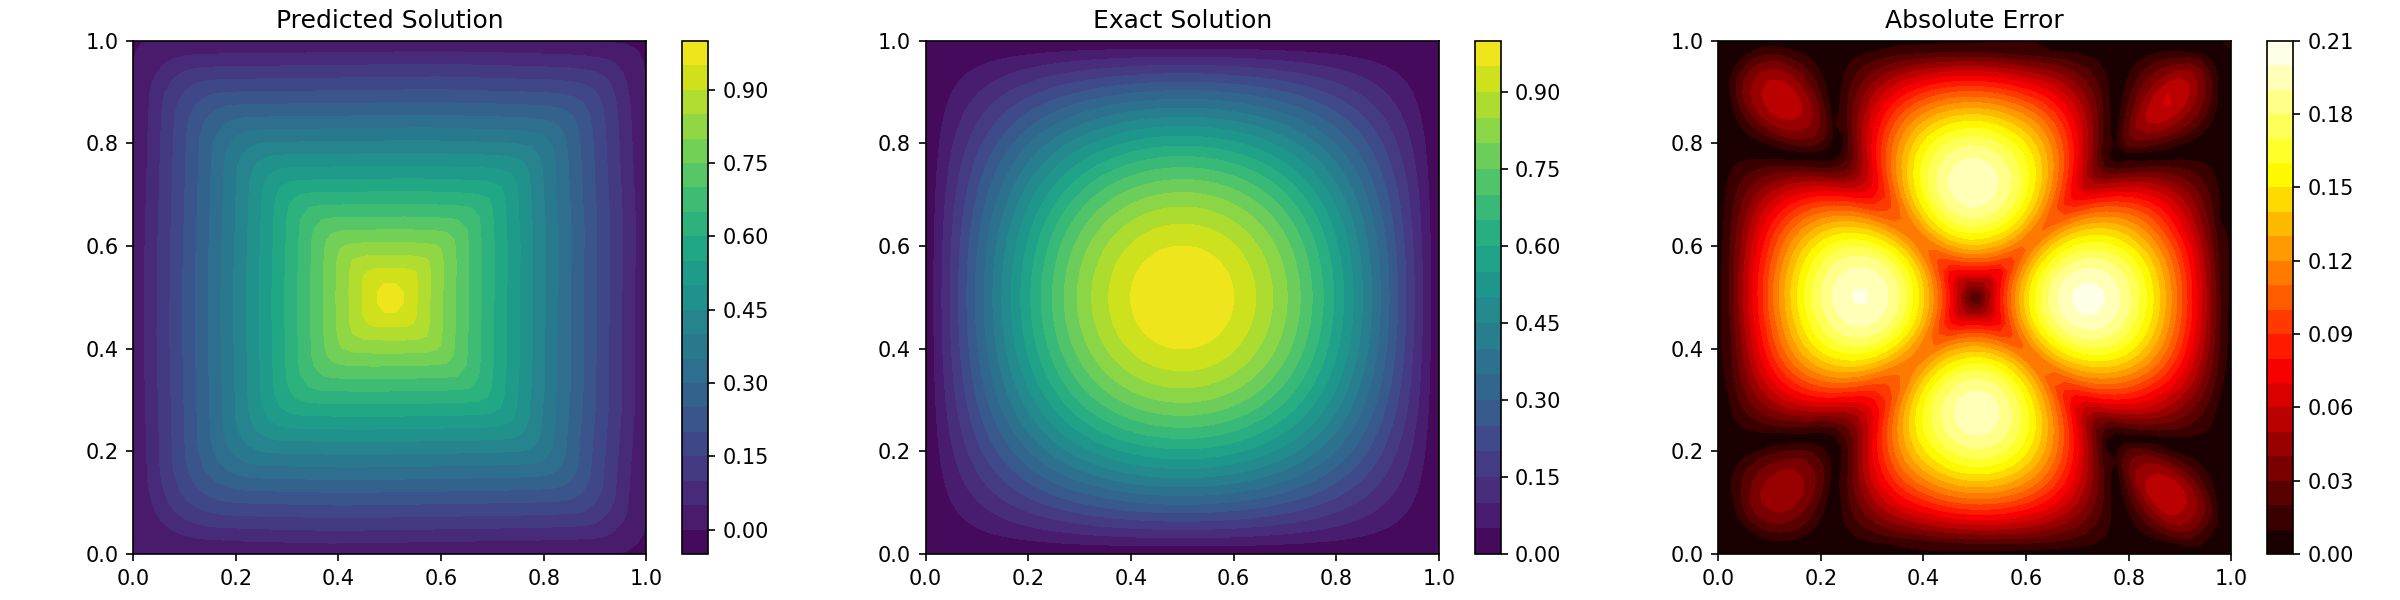
\includegraphics[width=\textwidth]{results/figures/solution_square_resnet.png}
    \caption{Deep Ritz数值解的可视化。(左)神经网络预测的解；(中)精确解；(右)绝对误差分布。误差分布表明网络很好地逼近了解析解，误差主要集中在边界附近。}
\end{figure}

\subsection{结构对比分析}

\subsubsection{ResNet vs 无ResNet对比}

两种网络结构的性能对比：

\begin{itemize}
  \item \textbf{无ResNet}：$L_2 = 8.762 \times 10^{-2}$，$L_\infty = 1.807 \times 10^{-1}$
  \item \textbf{ResNet}：$L_2 = 1.004 \times 10^{-1}$，$L_\infty = 2.037 \times 10^{-1}$
\end{itemize}

有趣的是，无ResNet版本在本实验中获得了略低的误差。这可能的原因包括：

\begin{enumerate}
  \item \textbf{问题复杂度}：该算例相对简单，简化的网络结构反而效率更高
  \item \textbf{网络容量}：ResNet的跳跃连接可能对这个问题引入了额外的约束
  \item \textbf{初始化影响}：网络参数初始化会影响收敛结果，导致随机波动
\end{enumerate}

然而，ResNet在更复杂的非线性PDE问题上通常表现更优，因为其能处理更深的网络而不产生梯度消失。

\setcounter{section}{6}
\section*{\centerline{六、关键技术讨论}}

\subsection{随机配点采样的重要性}

\textbf{随机配点 vs 固定配点的对比}：

\begin{enumerate}
  \item \textbf{过拟合}：固定配点的网络可能仅在采样点精确，在其他位置不精确
  \item \textbf{蒙特卡洛无偏性}：随机采样的积分估计渐近无偏，精度可由大数定律保证
  \item \textbf{批处理效率}：小批量随机采样可降低内存开销，提高GPU利用率
  \item \textbf{理论保证}：随机采样方法具有更好的泛化性能和收敛性
\end{enumerate}

在本方法中使用随机配点采样是算法的关键特性之一。

\subsection{罚参数的选择}

边界罚项系数$\beta$的影响：

\begin{equation}
L = L_{\text{interior}} + \beta L_{\text{boundary}}
\end{equation}

\begin{itemize}
  \item \textbf{$\beta$过小}（如$\beta < 1$）：边界条件约束不足，$u_\theta$在边界处不能很好满足$g(x)$
  \item \textbf{$\beta$适中}（$\beta \approx 100$-$1000$）：两项得到良好平衡
  \item \textbf{$\beta$过大}（$\beta > 10000$）：过度惩罚可能导致内部精度下降，或数值不稳定
\end{itemize}

本实验选择$\beta = 1000$，在保证边界条件满足和内部精度之间达到了较好的平衡。

\setcounter{section}{7}
\section*{\centerline{七、结论与展望}}

\subsection{主要发现}

\begin{enumerate}
  \item \textbf{可行性验证}：Deep Ritz方法成功求解了Poisson方程，数值误差在可接受范围内
  \item \textbf{无网格优势}：相比传统FEM/FDM，Deep Ritz无需网格生成，对复杂几何更友好
  \item \textbf{结构影响}：不同网络结构（有/无ResNet）对精度和收敛性都有影响
  \item \textbf{参数敏感性}：罚参数、学习率等超参数对结果质量重要，需仔细调优
\end{enumerate}

\subsection{方法优点}

\begin{enumerate}
  \item 无需生成复杂网格
  \item 易于扩展到非凸和复杂几何域
  \item 神经网络的可微性使导数计算便利
  \item 可并行化，适合GPU加速
\end{enumerate}

\subsection{方法不足}

\begin{enumerate}
  \item 单次计算成本（前向/反向传播）高于传统方法
  \item 需调整多个超参数（网络结构、学习率、罚参数等）
  \item 高维问题面临维数诅咒
  \item 缺乏完整的理论收敛性分析
\end{enumerate}

\subsection{改进与展望}

\begin{enumerate}
  \item \textbf{自适应采样}：在误差大的区域增加采样点密度
  \item \textbf{多物理耦合}：将PDE残差约束编入网络（如PINNs）
  \item \textbf{多尺度方法}：结合不同尺度特征改进高频分量
  \item \textbf{应用拓展}：非线性PDE、反演问题、参数优化等
\end{enumerate}

Deep Ritz方法代表了神经网络与科学计算的重要结合方向，有望在处理复杂工程问题中发挥重要作用。

\bibliographystyle{ieeetr}
\bibliography{refer}

\end{document}
